\documentclass[10pt]{article}

\usepackage{fullpage}
\usepackage{color}
\usepackage[table]{xcolor}
\usepackage{hyperref}
\usepackage{graphicx}
\usepackage{float}

%%%%%%%%%%%%%%%%
% Miscellaneous
%%%%%%%%%%%%%%%%

\definecolor{primary}{rgb}{0,0,.50}
%\definecolor{primary}{rgb}{0,0,0}
\definecolor{secondary}{rgb}{.7,.5,0}
\definecolor{table-primary}{rgb}{1,1,1}
\definecolor{table-secondary}{rgb}{.975,.99,1}
\setlength\fboxsep{0pt}
\setlength\fboxrule{0.5pt}

%%%%%%%%%%%%%%%%
% Title Section
%%%%%%%%%%%%%%%%

\title{\color{primary}\texttt{UCSC Plaza \\ User Manual}}
\author{{\color{secondary}\textbf{Team Amlesh the Great}} \\ Kyungmin So (PO), Youngsoo Jang, \\ Hobin Ryu, Seungwoo Lee \\ Amlesh Sivanantham, and James Garbagnati }
\date{Release: American Bobtail (July 25, 2016) \\ Release 1.0 (July 11, 2016)}

%%%%%%%%%%%%%%%%%%%%%%
% User-Defined Macros
%%%%%%%%%%%%%%%%%%%%%%

%\ignore = Multiline comments
\newcommand{\ignore}[1]{}

\newcommand{\gobblepagenum}{\thispagestyle{empty}\addtocounter{page}{-1}}

%\fancysec{Section title}{Label} = Fancy, colored and labelled section
% Basically just to make it easier to change the format of the whole doc
% Commands with an X are non-numbered sections
\newcommand{\fancysec}[2] {{\color{primary}\section{#1} \label{sec:#2}}}
\newcommand{\fancysub}[2] {{\color{primary}\subsection{#1} \label{sec:#2}}}
\newcommand{\fancysubsub}[2] {{\color{primary}\subsubsection{#1} \label{sec:#2}}}

\newcommand{\fancysecX}[2] {{\color{primary}\section*{#1} \label{sec:#2}}}
\newcommand{\fancysubX}[2] {{\color{primary}\subsection*{#1} \label{sec:#2}}}
\newcommand{\fancysubsubX}[2] {{\color{primary}\subsubsection*{#1} \label{sec:#2}}}

\newenvironment{captionedImage}[2]{
	\begin{figure}[H]
		\centering
		\fbox{\includegraphics[width=#2\textwidth]{}{}}
		\caption{#1}
		\label{fig:awesome_image}
	\end{figure}
}


% P.S. I'm so fancy, you already know


%%%%%%%%%%%%%%%%%
% Begin Document
%%%%%%%%%%%%%%%%%
\begin{document}
	
	\begin{titlepage}
		\centering
		
\includegraphics[width=0.45\textwidth]{logo}\par\vspace{1cm}
		{\scshape\LARGE Release 1.0 \par}
		\vspace{1.5cm}
		{\huge\bfseries\color{primary} User Manual\par}
		\vspace{2cm}
		{\Large\itshape Team Amlesh the Great\par}
		\vfill
		Team Members:\par
		Kyungmin So (Product Owner)\par 
		Youngsoo Jang\par 
		Hobin Ryu\par 
		Seungwoo Lee\par 
		Amlesh Sivanantham\par 
		James Garbagnati
		
		\vfill
		
		% Bottom of the page
		{\large \today\par}
	\end{titlepage}
	\hypersetup{%
		pdfborder = {0 0 0}
	}
	\large\tableofcontents
	\clearpage
	
	\fancysec{Introduction}{intro}
		UCSC Plaza is a event manager designed members of UCSC. This application has been tested on the Chromium browser. Other browsers are not guaranteed to work at this time. I'll probably put a more detailed description here eventually and also have a good overview picture here.
	
	
	\fancysec{Getting Started}{getstarted}
		\fancysub{Login Page}{loginpage}
			The first page we see when accessing the website is the login page.
			
			\begin{figure}[H]
				\centering
				\fbox{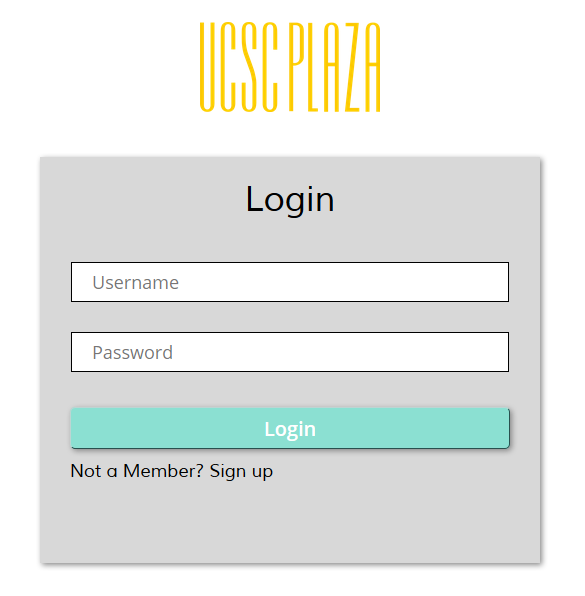
\includegraphics[width=0.7\textwidth]{loginPage}}
				\caption{Login Page}
				\label{fig:awesome_image}
			\end{figure}
			
			If you have already registered an account with us, please type your Username along with your Password and press the login button. You will now be taken to the main page. If you have not created an account with us, please click on the sign-up link below the login button to be redirected to the sign-up page. 
		
		\clearpage
		\fancysub{Sign-Up Page}{signup}
			The first step to signing up is choosing a username. Once you have typed a suitable username, press the "Check Duplication" button that is positioned directly right of it. If someone has taken your username, you will be notified that it has been taken. Otherwise, you will be notified that you can use this username.
			
			\begin{figure}[H]
				\centering
				\fbox{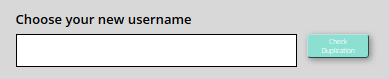
\includegraphics[width=0.7\textwidth]{signupUsername}}
				\caption{Username Prompt}
				\label{fig:awesome_image}
			\end{figure}			
			
			The next step is to make a strong password. After you have thought of a suitable password, please enter it into the "Create a password" field and make sure you retype the same password into the "Confirm your password" field as well.
			
			\begin{figure}[H]
				\centering
				\fbox{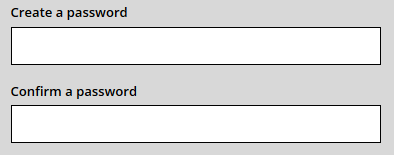
\includegraphics[width=0.7\textwidth]{signupPassword}}
				\caption{Password Prompt}
				\label{fig:awesome_image}
			\end{figure}		
			
			Its now time to personalize your account. The next section in the Sign-up Page will ask you for your first and last name along with your Major and Division. Please enter the correct responses.

			\begin{figure}[H]
				\centering
				\fbox{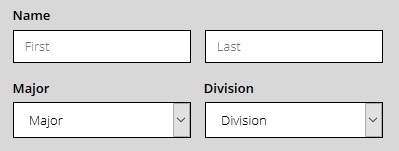
\includegraphics[width=0.7\textwidth]{signupDetails}}
				\caption{Password Prompt}
				\label{fig:awesome_image}
			\end{figure}	
			
			Finally, the last step before you can register your account is to verify your ucsc email. Once you have typed your email, please press the "Verify My Email" button. An email will be sent to your ucsc email address with a private key. The sign-up page will then ask for you to type your private key. Please do so and then press the "Verify" button to continue. If you typed out the key correctly, you can then proceed onward. If your key did not work, check to see if you misspelled it and try again.
				
			\begin{figure}[H]
				\centering
				\fbox{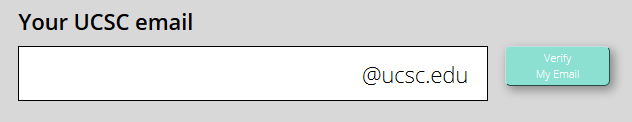
\includegraphics[width=0.7\textwidth]{signupEmailBefore}}
				\caption{Email Prompt Before}
				\label{fig:awesome_image}
			\end{figure}
			
			\begin{figure}[H]
				\centering
				\fbox{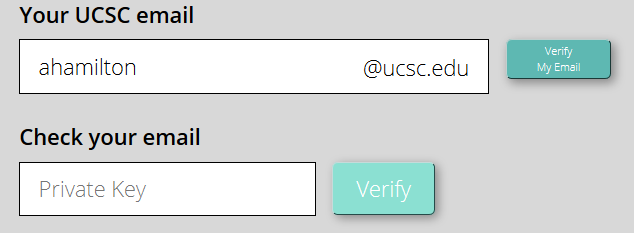
\includegraphics[width=0.7\textwidth]{signupEmailAfter}}
				\caption{Email Prompt After}
				\label{fig:awesome_image}
			\end{figure}
			
			If you have done all these steps correctly, you can finish creating your account by pressing the "Confirm" button. Doing so will create your account and take you back to the Login page.
	
	\clearpage		
	\fancysec{Adding and Viewing to Events}{viewrespondevents}
		\fancysub{Viewing Events}{viewevent}
			Seen below is the Main Page. This is where you can view and search for events happening at UCSC. You can always come back to this page by clicking the UCSC Plaza logo on the top left of the page. To the left you can see a listing for events happening at UCSC. Their locations on marked on the google map. Furthermore if you hover over an event, the respective marker will bounce on the map!
			
			\begin{figure}[H]
				\centering
				\fbox{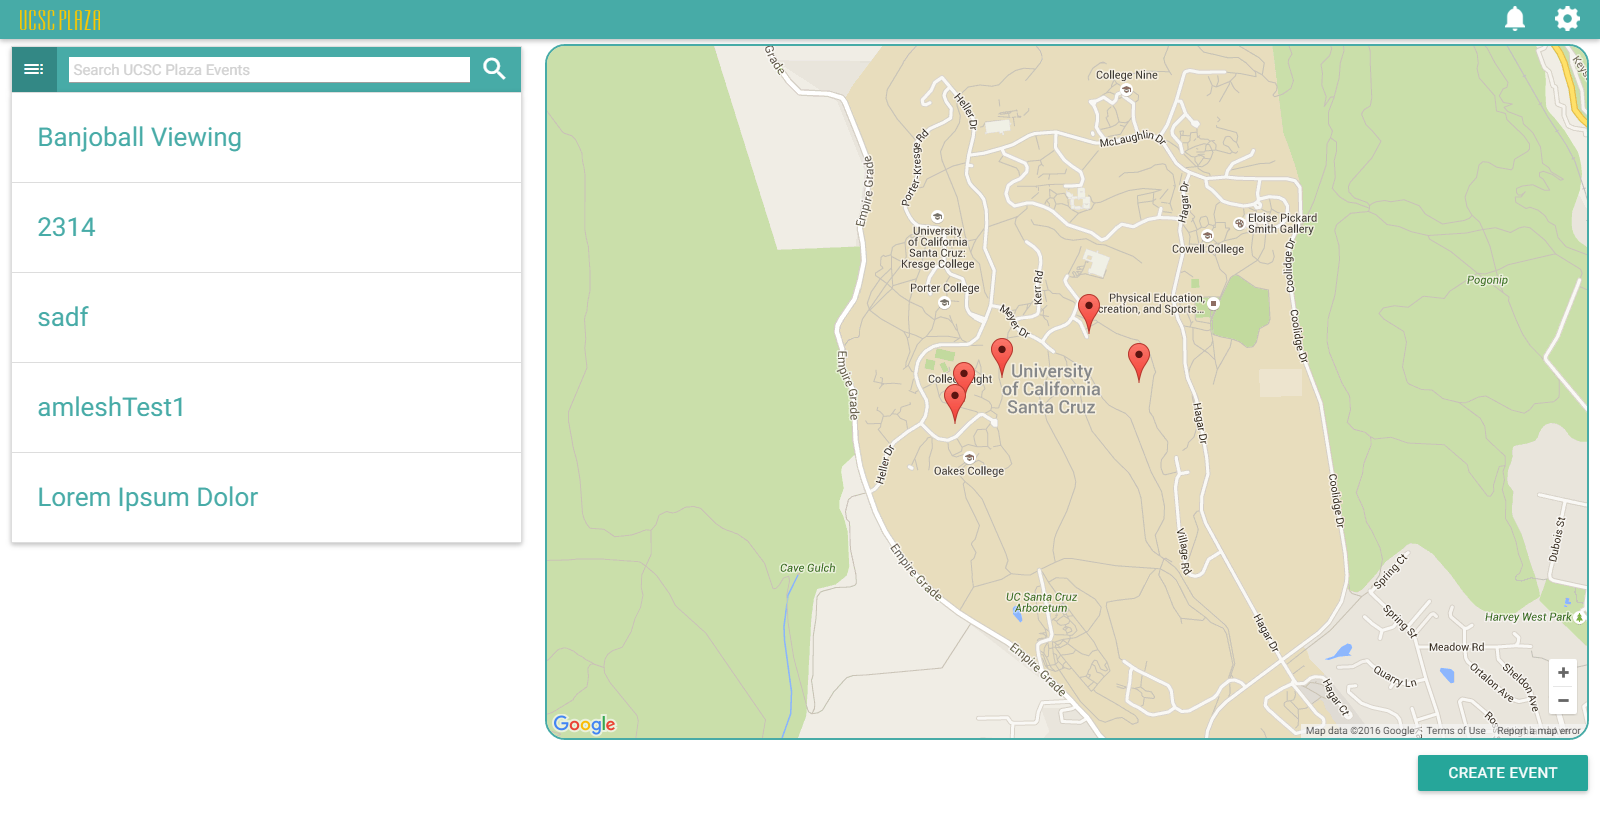
\includegraphics[width=0.7\textwidth]{mainPage}}
				\caption{Main Page}
				\label{fig:awesome_image}
			\end{figure}
			
			To start searching for specific events, you can type your search in the search bar above. You can get really specific with your search by clicking on the button directly left of the search bar. It will open up the Search Menu. You can use this menu to search under specific conditions. The search menu does not appear to work in this current implementation.
			
			\begin{figure}[H]
				\centering
				\fbox{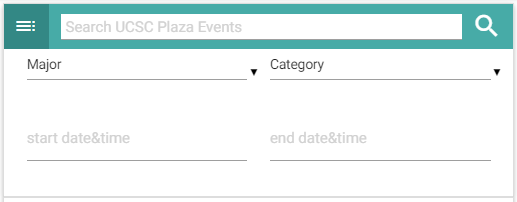
\includegraphics[width=0.7\textwidth]{searchMenu}}
				\caption{Search Menu}
				\label{fig:awesome_image}
			\end{figure}
			
			Once you have found an event that interests you, you can click on it to pull the expanded view. This view will give you more information about an event. You can see from the figure below, That there are alot of details present. Let's go over them now.\par 
			
			\begin{figure}[H]
				\centering
				\fbox{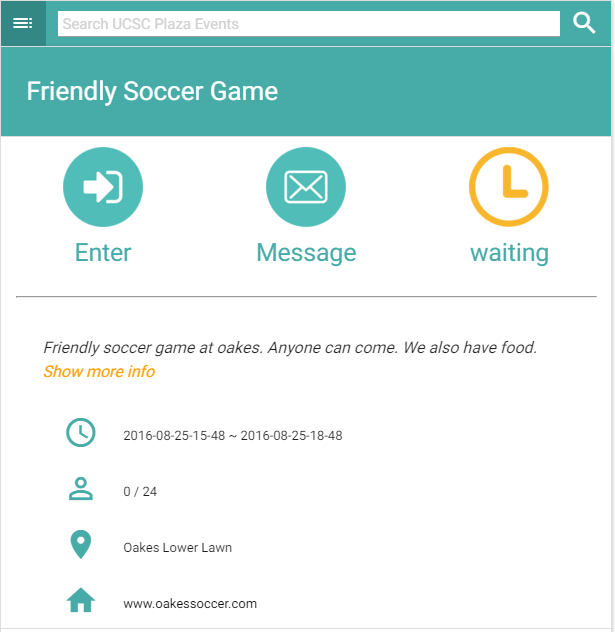
\includegraphics[width=0.6\textwidth]{eventExpand}}
				\caption{Expanded View}
				\label{fig:awesome_image}
			\end{figure}
			
			The first thing we see are three icons. These icons are the Enter, Message, and Waiting buttons. The Enter icon is a button that sends your related info to the host and tells them that you are interested in this event. By clicking on this button, you can apply for this event. You will notice that the icon changes to a red icon saying Leave which you can see in the Figure below. You can press this icon again to leave any events you have applied to.\par
			
			\begin{figure}[H]
				\centering
				\fbox{
\includegraphics[width=0.4\textwidth]{eventExpandLeave}}
				\caption{After you apply to an Event, you have the option to leave.}
				\label{fig:awesome_image}
			\end{figure}			 
			
			Unfortunately, this Release of UCSC Plaza does not support the message button. The purpose of this button is to message the host. The final icon is the waiting icon. It represents your current status for the event. If the host has approved your application for the event, that icon changes to approved icon. You can see this in the figure below.
			
			\begin{figure}[H]
				\centering
				\fbox{\includegraphics[width=0.4\textwidth]{eventExpandAccepted}}
				\caption{The host has accepted you to their event.}
				\label{fig:awesome_image}
			\end{figure}
			
			You can take a look at figure 9 again and you will notice that under these icons, there are some details of a description, time of the event, current and max attendance of an event, the location of the event, and the event's homepage. If we click the highlighted "Show more info" text, we will be taken to the Detailed view. This is a window that pops up in the current view, but shows a bit more info, including a picture that the host may have uploaded for an event. This can be seen in the figure below.
			
			\begin{figure}[H]
				\centering
				\fbox{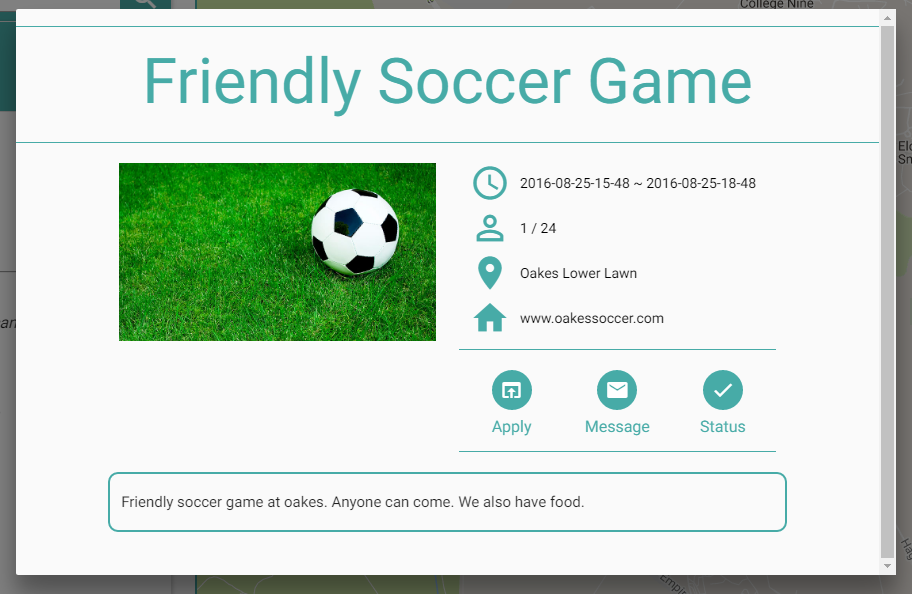
\includegraphics[width=0.7\textwidth]{eventDetailedView}}
				\caption{Detailed View}
				\label{fig:awesome_image}
			\end{figure}	
			
			The last thing you should know about is that you can all see any event that you are also hosting in this listing. If you click on the event, you can see only one icon in the expanded view. This is the option to delete your event.You can see it for yourself in the figure below. You can also do this in your page, which we will cover in the My Page section.
			
			\begin{figure}[H]
				\centering
				\fbox{
\includegraphics[width=0.4\textwidth]{eventExpandDelete}}
				\caption{Delete  Event}
				\label{fig:awesome_image}
			\end{figure}			
			
		\clearpage
		\fancysub{Adding Events}{addevent}
			Here is an overview of the Add Event page. We will get into detail as to what each field means.
			\begin{figure}[H]
				\centering
				\fbox{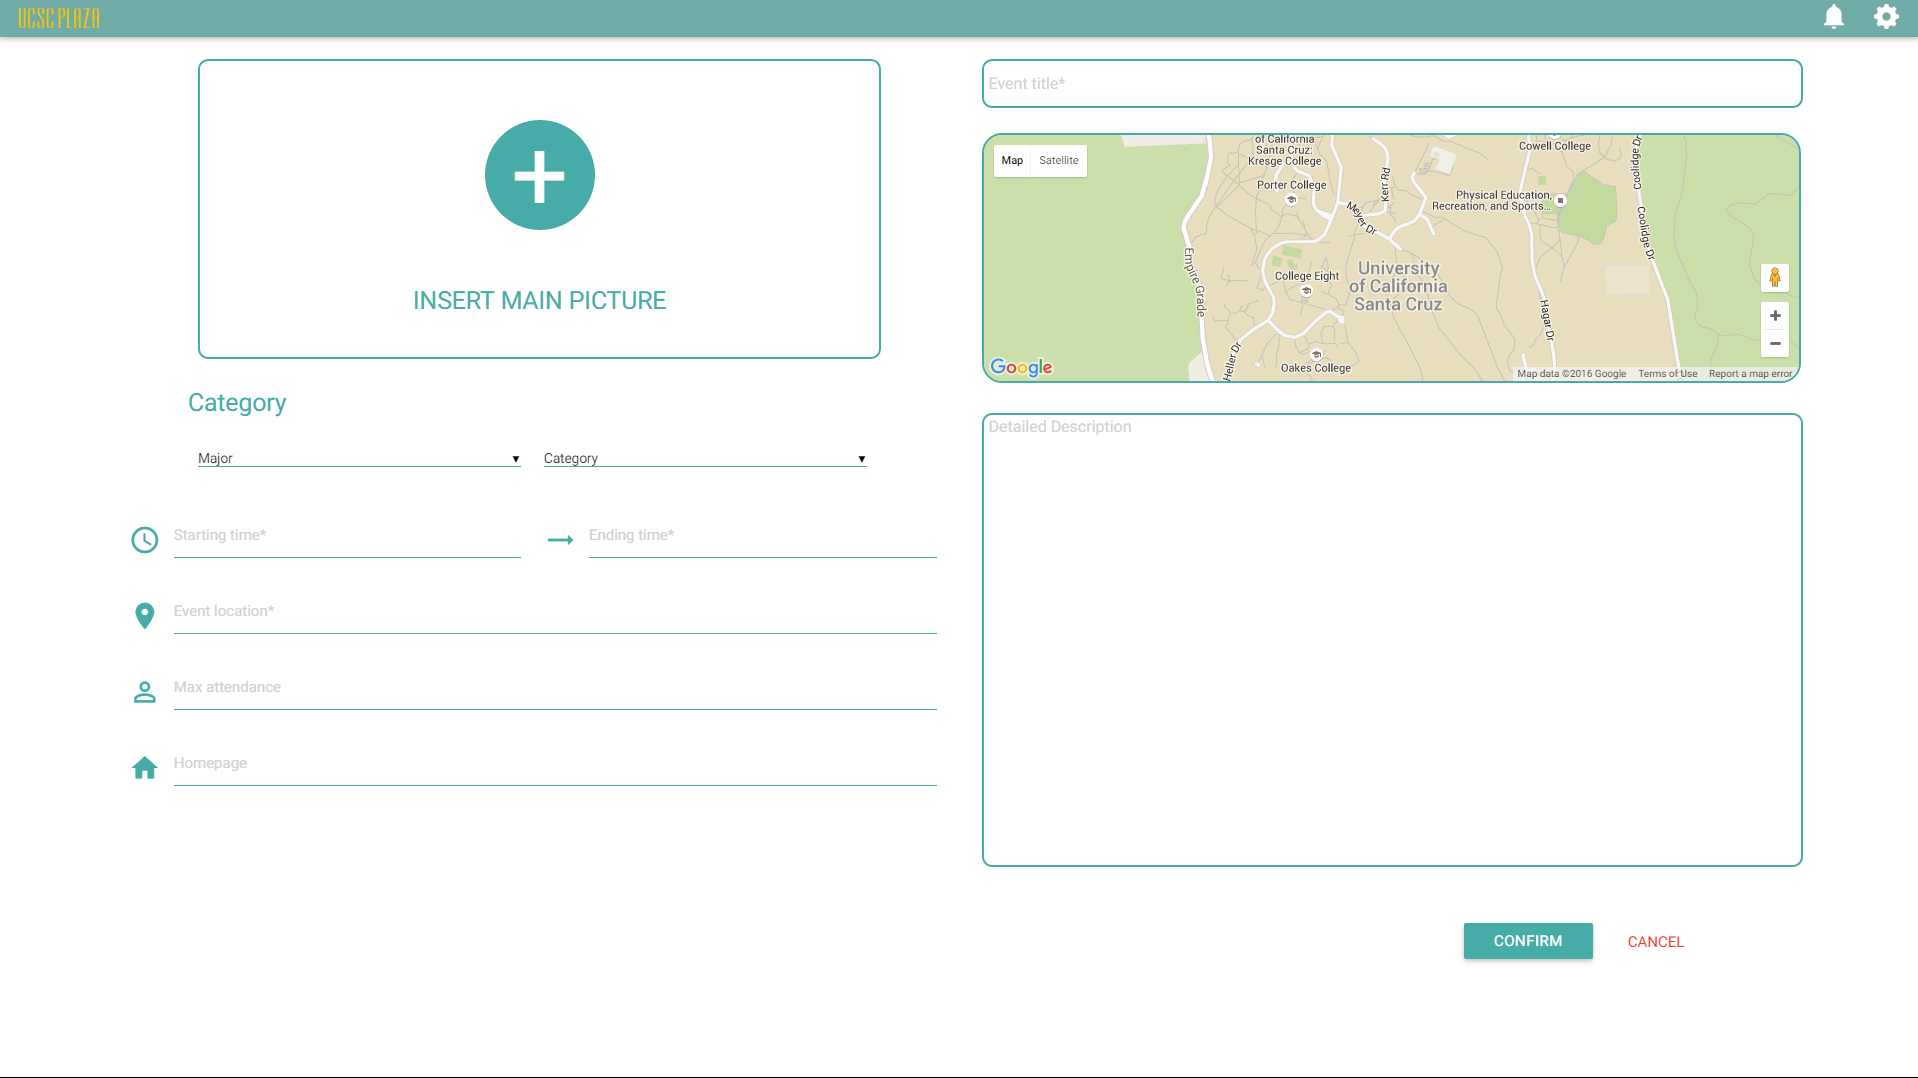
\includegraphics[width=0.9\textwidth]{addEventFull}}
				\caption{Email Prompt After}
				\label{fig:awesome_image}
			\end{figure}
			
			The first input fields we will look at is the Event Title and Google Map View. Simply type the title of your event into the Event Title field. To place a marker on the google map, simply click on the location you wish to mark. This is demonstrated in Figure number. The Google Map view can be zoomed in and out using the mouse scroll wheel, it can also be moved around by clicking an area and dragging the mouse.

			\begin{figure}[H]
				\centering
				\fbox{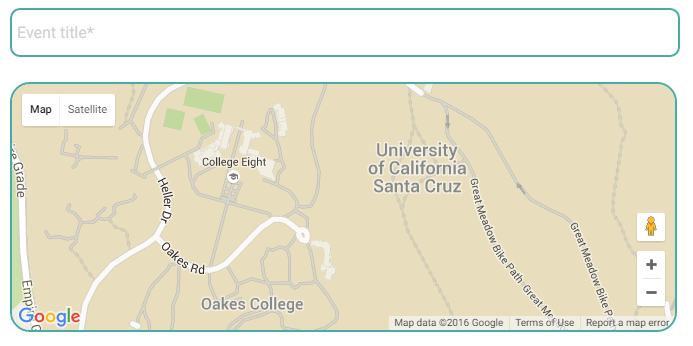
\includegraphics[width=0.6\textwidth]{addEventTitle}}
				\caption{Adding Event Title and Marker Location}
				\label{fig:awesome_image}
			\end{figure}

			
			\begin{figure}[H]
				\centering
				\fbox{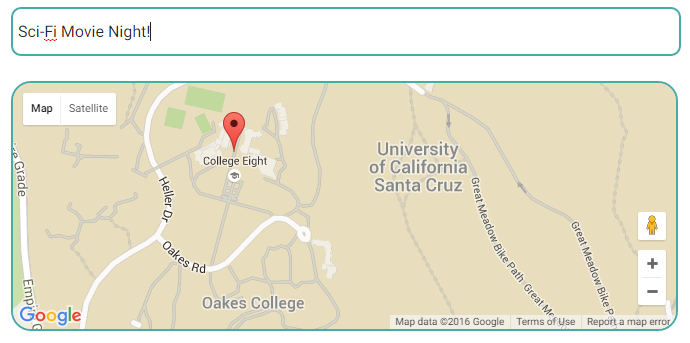
\includegraphics[width=0.6\textwidth]{eventMarkerOn}}
				\caption{Here is the map with the Marker Location set}
				\label{fig:awesome_image}
			\end{figure}
			
			Directly below these two fields, there is a Detailed Description input field. Please feel free to add more information about your event here.\\
			
			\par You can also add a picture that to represent your event. Simply click on the INSERT MAIN PICTURE button and select your file. You are only allowed to upload image files.

			\begin{figure}[H]
				\centering
				\fbox{
\includegraphics[width=0.6\textwidth]{eventAddImage}}
				\caption{Select this button to add an image}
				\label{fig:awesome_image}
			\end{figure}
			
			You can now choose which Categories and what Academic Major you believe best describes your Event. Seen below is a dropdown view of both the categories and major selection lists.
			
			 \begin{figure}[H]
			 	\centering
			 	\fbox{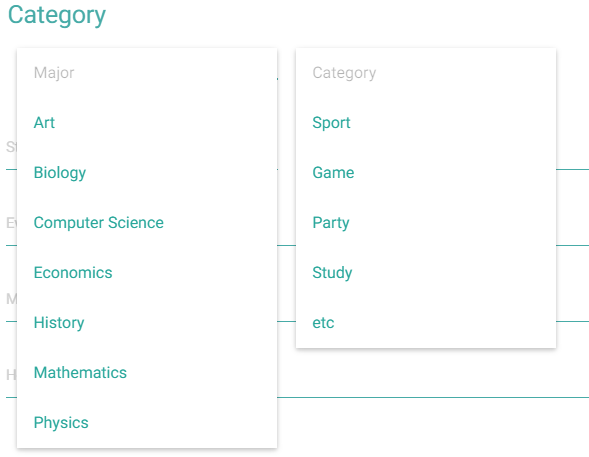
\includegraphics[width=0.5\textwidth]{addEventCat}}
			 	\caption{Please select an option in each of these fields}
			 	\label{fig:awesome_image}
			 \end{figure}
			 
			 All thats left for you is to give the finer details of your event. This includes the Start Time and End Time, the Location, the Max Attendance, and the Homepage.
			 
			  \begin{figure}[H]
			  	\centering
			  	\fbox{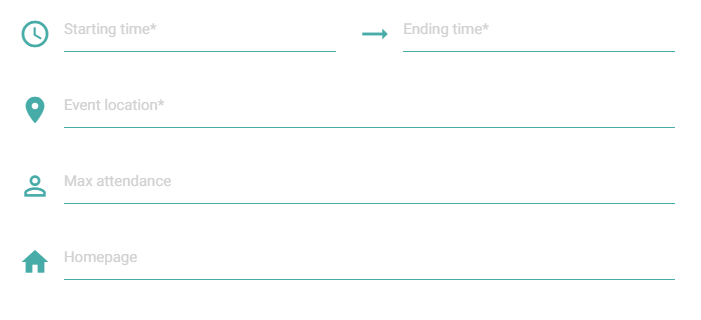
\includegraphics[width=0.6\textwidth]{addEventOther}}
			  	\caption{The finer details of your event}
			  	\label{fig:awesome_image}
			  \end{figure}
			  
			  It should be noted however that the Start Time, End Time, and Location are the only required fields. The Hompage and Max Attendance can be left blank. \\
			  \par Once you are all done setting up the details of your Event, hit the Confirm button at the bottom of the page. If you answered all the required fields, your event will be added to the database. If you wish to not upload the event you just made, press the cancel button instead and you will be taken back to the main page.
			
			  \begin{figure}[H]
			  	\centering
			  	\fbox{
\includegraphics[width=0.3\textwidth]{addEventButton}}
			  	\caption{Choose to upload the Event or cancel the action}
			  	\label{fig:awesome_image}
			  \end{figure}
	
	\clearpage
	\fancysec{My Page}{mypage}
		\fancysub{Your Events}{uevents}
		
			To view your page, click the gear icon. A selection option called "My Page" should appear. Click on it to be redirected to the My Page. Seen below is an overview of what you My Page may look like. To the right, there is a grey box with some of your personal details on it that you gave to us during account creation.
		
			\begin{figure}[H]
				\centering
				\fbox{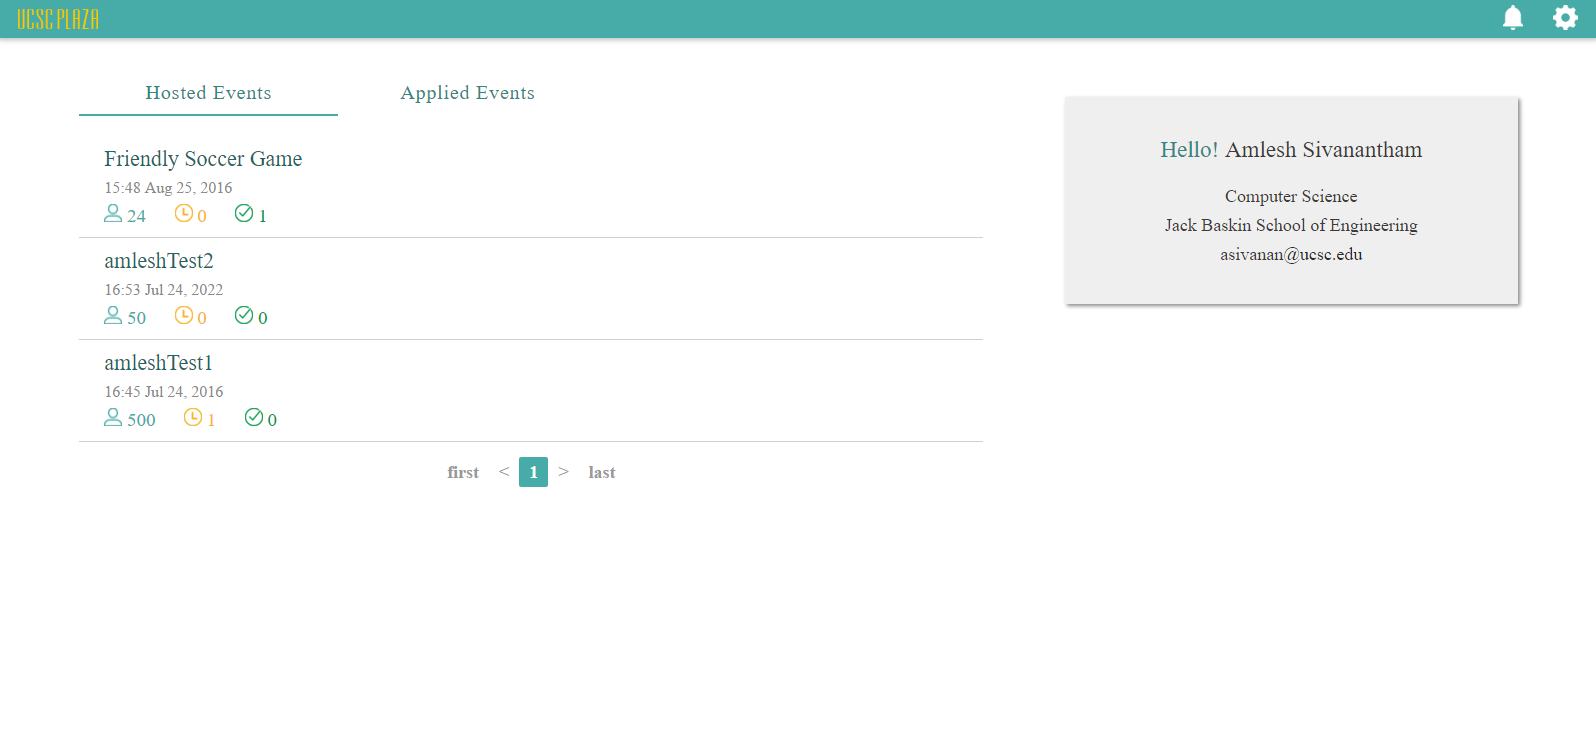
\includegraphics[width=0.8\textwidth]{myPage}}
				\caption{My Page}
				\label{fig:awesome_image}
			\end{figure}	
			
			The first thing we will bring our attention to is the two tabs, labeled "Hosted Events" and "Applied Events". The My Page defaults to loading the "Hosted Events" tab and that will be the focus of this section. The "Applied Events" tab will be the focus of the next section.
		
			\begin{figure}[H]
				\centering
				\fbox{
\includegraphics[width=0.8\textwidth]{myPageTabs}}
				\caption{My Page Tabs}
				\label{fig:awesome_image}
			\end{figure}		
			
			Unlike the event listing in the Main Page, this event list is not scrollable, but you can use the arrow keys in the bottom to move through the event listing. \par 
			Lets take a look at what details are shown. We can see the event title, start date of the event, and a couple other numbers. This can be seen in the figure below.
			
			\begin{figure}[H]
				\centering
				\fbox{
\includegraphics[width=0.8\textwidth]{myPageEvent}}
				\caption{My Page Event}
				\label{fig:awesome_image}
			\end{figure}
			
			The number beside the person icon signifies the max attendance for that event. The number beside the clock icon shows the number of people waiting to be accepted to the event, and the number beside the green check mark is the number of people you have accepted. Clicking on the event will pull up a list of users that are interested in your event. It defaults to opening the Waiting Tab.
			
			\begin{figure}[H]
				\centering
				\fbox{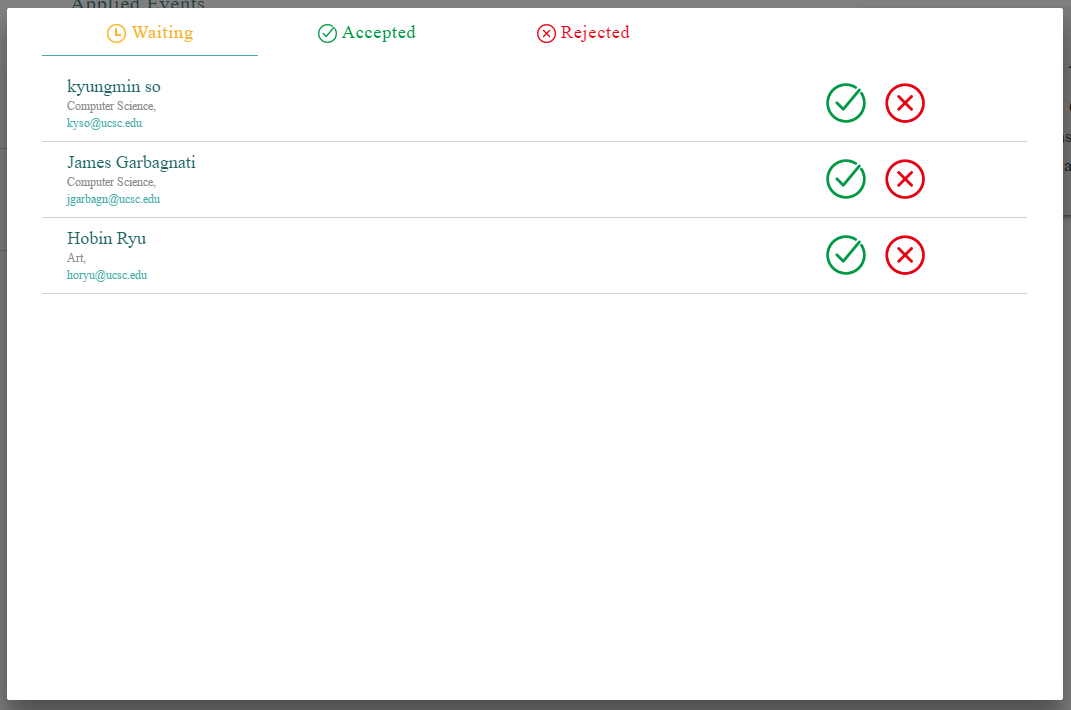
\includegraphics[width=0.8\textwidth]{myPageEventPeople}}
				\caption{Users Interested in your Event}
				\label{fig:awesome_image}
			\end{figure}
			
			Beside each person's name are a green checkmark and a red x-mark. You can accept and decline these users by pressing these buttons. You can see the users you have accepted by clicking the Accepted tab, and you can view the users you have rejected by clicking the Rejected tab.
			
			\begin{figure}[H]
				\centering
				\fbox{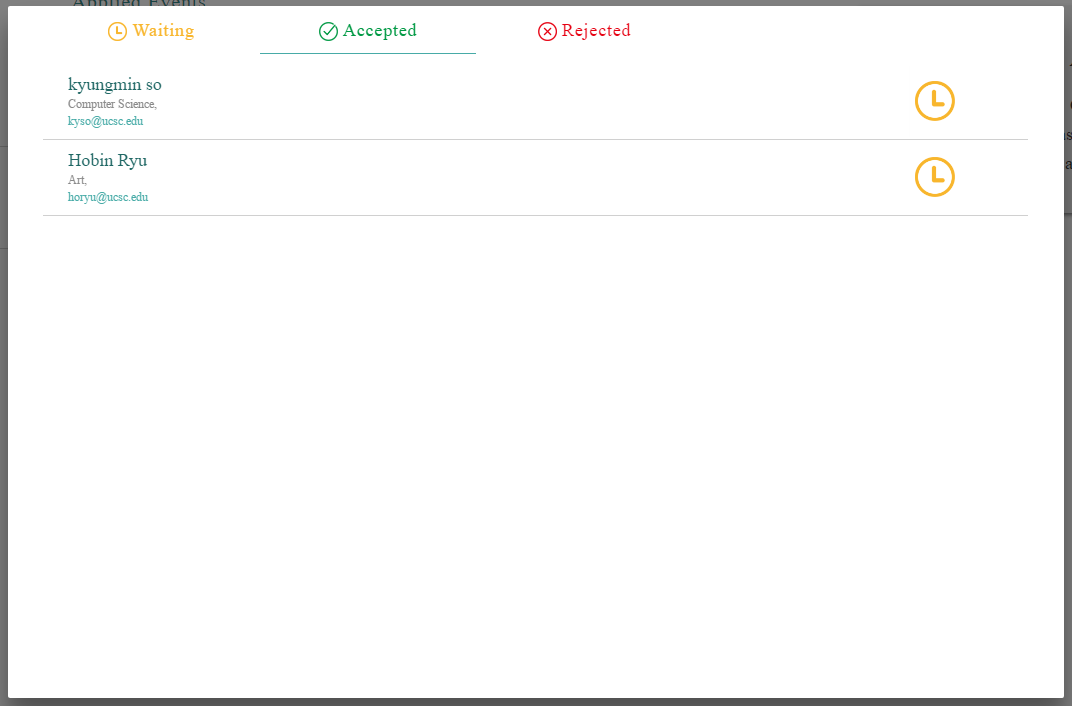
\includegraphics[width=0.7\textwidth]{myPageEventPeopleAccepted}}
				\caption{Your Accepted Users}
				\label{fig:awesome_image}
			\end{figure}
			
			\begin{figure}[H]
				\centering
				\fbox{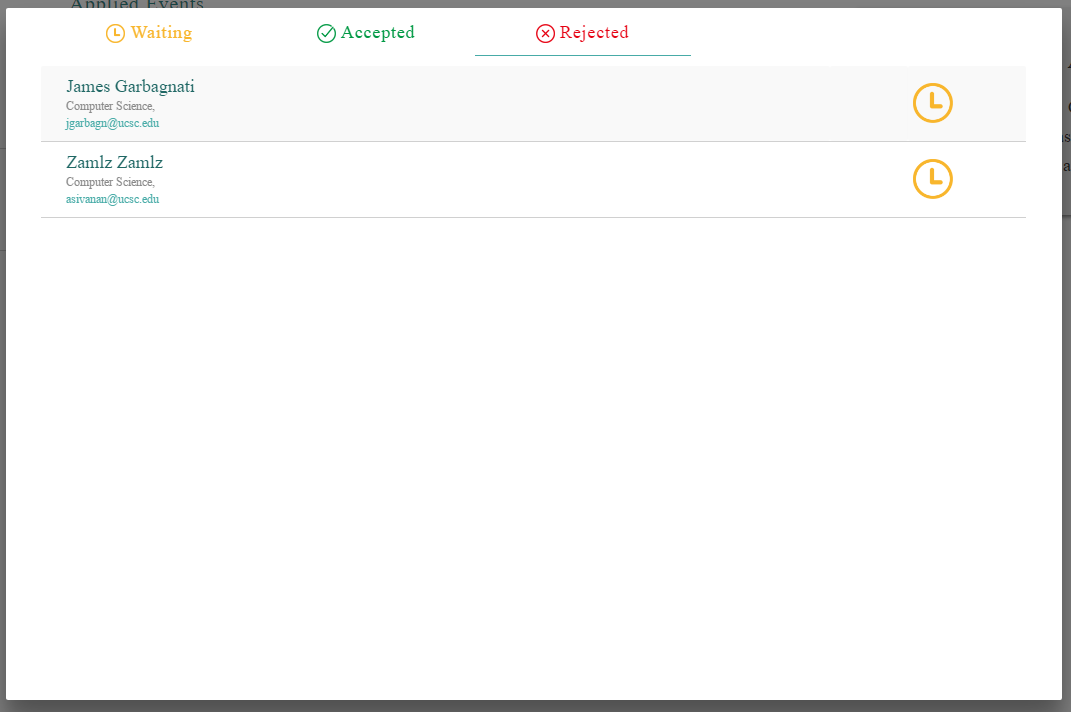
\includegraphics[width=0.7\textwidth]{myPageEventPeopleRejected}}
				\caption{Your Rejected Users}
				\label{fig:awesome_image}
			\end{figure}
		
			In both of these tabs, you can send the user back to the waiting tab by selecting the yellow clock button. Then, simply switch to the Waiting tab again to decide whether you should accept or reject them.
		
		\clearpage
		\fancysub{Applied Events}{aevents}
			If you switch to the Applied Events tab, you will notice that the event list view has changed. Instead of showing the number of people who have applied, got accepted, etc., it instead shows us the owner of the event. To right of that event, you can see your accepted status. You can either have waiting icon, rejected icon, or an accepted icon. You can see an example below.
			
			\begin{figure}[H]
				\centering
				\fbox{
\includegraphics[width=0.8\textwidth]{myPageApplied}}
				\caption{My Page , Applied Events}
				\label{fig:awesome_image}
			\end{figure}
			
			If you click on the event, it will pull up the detailed view. From here, you can choose to leave the event if necessary.
\end{document}
